% Created by tikzDevice version 0.12.3.1 on 2023-05-05 12:20:06
% !TEX encoding = UTF-8 Unicode
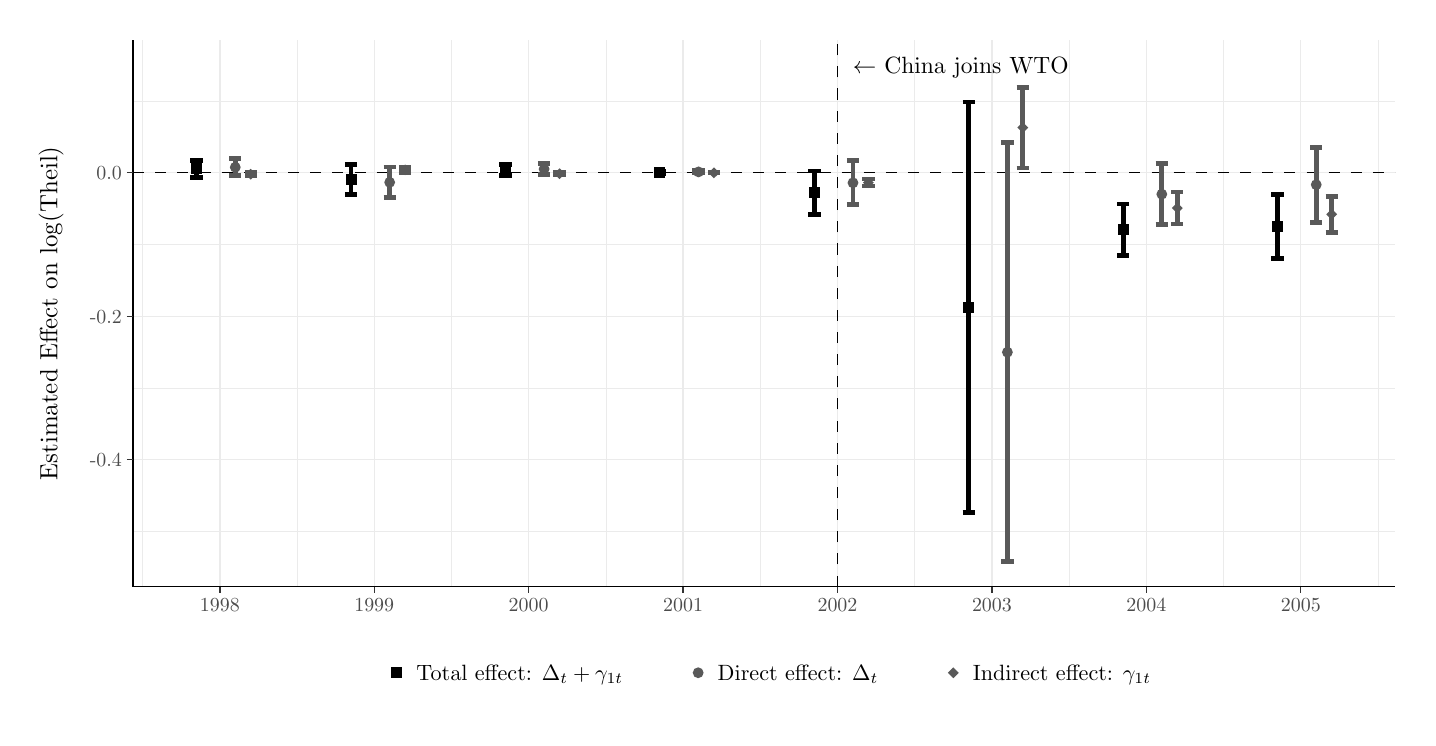
\begin{tikzpicture}[x=1pt,y=1pt]
\definecolor{fillColor}{RGB}{255,255,255}
\path[use as bounding box,fill=fillColor] (0,0) rectangle (498.66,249.33);
\begin{scope}
\path[clip] (  0.00,  0.00) rectangle (498.66,249.33);
\definecolor{drawColor}{RGB}{255,255,255}

\path[draw=drawColor,line width= 0.5pt,line join=round,line cap=round,fill=fillColor] ( -0.00,  0.00) rectangle (498.66,249.33);
\end{scope}
\begin{scope}
\path[clip] ( 38.10, 47.36) rectangle (494.16,244.83);
\definecolor{fillColor}{RGB}{255,255,255}

\path[fill=fillColor] ( 38.10, 47.36) rectangle (494.16,244.83);
\definecolor{drawColor}{gray}{0.92}

\path[draw=drawColor,line width= 0.2pt,line join=round] ( 38.10, 67.25) --
	(494.16, 67.25);

\path[draw=drawColor,line width= 0.2pt,line join=round] ( 38.10,119.13) --
	(494.16,119.13);

\path[draw=drawColor,line width= 0.2pt,line join=round] ( 38.10,171.01) --
	(494.16,171.01);

\path[draw=drawColor,line width= 0.2pt,line join=round] ( 38.10,222.89) --
	(494.16,222.89);

\path[draw=drawColor,line width= 0.2pt,line join=round] ( 41.53, 47.36) --
	( 41.53,244.83);

\path[draw=drawColor,line width= 0.2pt,line join=round] ( 97.33, 47.36) --
	( 97.33,244.83);

\path[draw=drawColor,line width= 0.2pt,line join=round] (153.13, 47.36) --
	(153.13,244.83);

\path[draw=drawColor,line width= 0.2pt,line join=round] (208.93, 47.36) --
	(208.93,244.83);

\path[draw=drawColor,line width= 0.2pt,line join=round] (264.73, 47.36) --
	(264.73,244.83);

\path[draw=drawColor,line width= 0.2pt,line join=round] (320.54, 47.36) --
	(320.54,244.83);

\path[draw=drawColor,line width= 0.2pt,line join=round] (376.34, 47.36) --
	(376.34,244.83);

\path[draw=drawColor,line width= 0.2pt,line join=round] (432.14, 47.36) --
	(432.14,244.83);

\path[draw=drawColor,line width= 0.2pt,line join=round] (487.94, 47.36) --
	(487.94,244.83);

\path[draw=drawColor,line width= 0.5pt,line join=round] ( 38.10, 93.19) --
	(494.16, 93.19);

\path[draw=drawColor,line width= 0.5pt,line join=round] ( 38.10,145.07) --
	(494.16,145.07);

\path[draw=drawColor,line width= 0.5pt,line join=round] ( 38.10,196.95) --
	(494.16,196.95);

\path[draw=drawColor,line width= 0.5pt,line join=round] ( 69.43, 47.36) --
	( 69.43,244.83);

\path[draw=drawColor,line width= 0.5pt,line join=round] (125.23, 47.36) --
	(125.23,244.83);

\path[draw=drawColor,line width= 0.5pt,line join=round] (181.03, 47.36) --
	(181.03,244.83);

\path[draw=drawColor,line width= 0.5pt,line join=round] (236.83, 47.36) --
	(236.83,244.83);

\path[draw=drawColor,line width= 0.5pt,line join=round] (292.63, 47.36) --
	(292.63,244.83);

\path[draw=drawColor,line width= 0.5pt,line join=round] (348.44, 47.36) --
	(348.44,244.83);

\path[draw=drawColor,line width= 0.5pt,line join=round] (404.24, 47.36) --
	(404.24,244.83);

\path[draw=drawColor,line width= 0.5pt,line join=round] (460.04, 47.36) --
	(460.04,244.83);
\definecolor{drawColor}{RGB}{0,0,0}

\path[draw=drawColor,line width= 0.6pt,dash pattern=on 4pt off 4pt ,line join=round] ( 38.10,196.95) -- (494.16,196.95);

\path[draw=drawColor,line width= 0.6pt,dash pattern=on 4pt off 4pt ,line join=round] (292.63, 47.36) -- (292.63,244.83);

\node[text=drawColor,anchor=base west,inner sep=0pt, outer sep=0pt, scale=  0.85] at (298.22,232.92) {$\leftarrow$ China joins WTO};

\path[draw=drawColor,line width= 1.7pt,line join=round] ( 58.83,201.34) --
	( 63.29,201.34);

\path[draw=drawColor,line width= 1.7pt,line join=round] ( 61.06,201.34) --
	( 61.06,195.30);

\path[draw=drawColor,line width= 1.7pt,line join=round] ( 58.83,195.30) --
	( 63.29,195.30);

\path[draw=drawColor,line width= 1.7pt,line join=round] (114.63,199.92) --
	(119.09,199.92);

\path[draw=drawColor,line width= 1.7pt,line join=round] (116.86,199.92) --
	(116.86,189.00);

\path[draw=drawColor,line width= 1.7pt,line join=round] (114.63,189.00) --
	(119.09,189.00);

\path[draw=drawColor,line width= 1.7pt,line join=round] (170.43,199.90) --
	(174.89,199.90);

\path[draw=drawColor,line width= 1.7pt,line join=round] (172.66,199.90) --
	(172.66,195.84);

\path[draw=drawColor,line width= 1.7pt,line join=round] (170.43,195.84) --
	(174.89,195.84);

\path[draw=drawColor,line width= 1.7pt,line join=round] (226.23,197.54) --
	(230.69,197.54);

\path[draw=drawColor,line width= 1.7pt,line join=round] (228.46,197.54) --
	(228.46,196.72);

\path[draw=drawColor,line width= 1.7pt,line join=round] (226.23,196.72) --
	(230.69,196.72);

\path[draw=drawColor,line width= 1.7pt,line join=round] (282.03,197.58) --
	(286.50,197.58);

\path[draw=drawColor,line width= 1.7pt,line join=round] (284.26,197.58) --
	(284.26,181.75);

\path[draw=drawColor,line width= 1.7pt,line join=round] (282.03,181.75) --
	(286.50,181.75);

\path[draw=drawColor,line width= 1.7pt,line join=round] (337.83,222.52) --
	(342.30,222.52);

\path[draw=drawColor,line width= 1.7pt,line join=round] (340.07,222.52) --
	(340.07, 74.18);

\path[draw=drawColor,line width= 1.7pt,line join=round] (337.83, 74.18) --
	(342.30, 74.18);

\path[draw=drawColor,line width= 1.7pt,line join=round] (393.64,185.61) --
	(398.10,185.61);

\path[draw=drawColor,line width= 1.7pt,line join=round] (395.87,185.61) --
	(395.87,167.10);

\path[draw=drawColor,line width= 1.7pt,line join=round] (393.64,167.10) --
	(398.10,167.10);

\path[draw=drawColor,line width= 1.7pt,line join=round] (449.44,189.17) --
	(453.90,189.17);

\path[draw=drawColor,line width= 1.7pt,line join=round] (451.67,189.17) --
	(451.67,165.88);

\path[draw=drawColor,line width= 1.7pt,line join=round] (449.44,165.88) --
	(453.90,165.88);
\definecolor{drawColor}{gray}{0.35}

\path[draw=drawColor,line width= 1.7pt,line join=round] ( 72.78,201.94) --
	( 77.24,201.94);

\path[draw=drawColor,line width= 1.7pt,line join=round] ( 75.01,201.94) --
	( 75.01,195.83);

\path[draw=drawColor,line width= 1.7pt,line join=round] ( 72.78,195.83) --
	( 77.24,195.83);

\path[draw=drawColor,line width= 1.7pt,line join=round] (128.58,198.96) --
	(133.04,198.96);

\path[draw=drawColor,line width= 1.7pt,line join=round] (130.81,198.96) --
	(130.81,187.91);

\path[draw=drawColor,line width= 1.7pt,line join=round] (128.58,187.91) --
	(133.04,187.91);

\path[draw=drawColor,line width= 1.7pt,line join=round] (184.38,200.30) --
	(188.84,200.30);

\path[draw=drawColor,line width= 1.7pt,line join=round] (186.61,200.30) --
	(186.61,196.20);

\path[draw=drawColor,line width= 1.7pt,line join=round] (184.38,196.20) --
	(188.84,196.20);

\path[draw=drawColor,line width= 1.7pt,line join=round] (240.18,197.63) --
	(244.65,197.63);

\path[draw=drawColor,line width= 1.7pt,line join=round] (242.41,197.63) --
	(242.41,196.79);

\path[draw=drawColor,line width= 1.7pt,line join=round] (240.18,196.79) --
	(244.65,196.79);

\path[draw=drawColor,line width= 1.7pt,line join=round] (295.98,201.23) --
	(300.45,201.23);

\path[draw=drawColor,line width= 1.7pt,line join=round] (298.22,201.23) --
	(298.22,185.31);

\path[draw=drawColor,line width= 1.7pt,line join=round] (295.98,185.31) --
	(300.45,185.31);

\path[draw=drawColor,line width= 1.7pt,line join=round] (351.78,207.78) --
	(356.25,207.78);

\path[draw=drawColor,line width= 1.7pt,line join=round] (354.02,207.78) --
	(354.02, 56.34);

\path[draw=drawColor,line width= 1.7pt,line join=round] (351.78, 56.34) --
	(356.25, 56.34);

\path[draw=drawColor,line width= 1.7pt,line join=round] (407.59,200.17) --
	(412.05,200.17);

\path[draw=drawColor,line width= 1.7pt,line join=round] (409.82,200.17) --
	(409.82,178.16);

\path[draw=drawColor,line width= 1.7pt,line join=round] (407.59,178.16) --
	(412.05,178.16);

\path[draw=drawColor,line width= 1.7pt,line join=round] (463.39,206.12) --
	(467.85,206.12);

\path[draw=drawColor,line width= 1.7pt,line join=round] (465.62,206.12) --
	(465.62,179.05);

\path[draw=drawColor,line width= 1.7pt,line join=round] (463.39,179.05) --
	(467.85,179.05);

\path[draw=drawColor,line width= 1.7pt,line join=round] ( 78.36,196.87) --
	( 82.82,196.87);

\path[draw=drawColor,line width= 1.7pt,line join=round] ( 80.59,196.87) --
	( 80.59,195.89);

\path[draw=drawColor,line width= 1.7pt,line join=round] ( 78.36,195.89) --
	( 82.82,195.89);

\path[draw=drawColor,line width= 1.7pt,line join=round] (134.16,198.85) --
	(138.62,198.85);

\path[draw=drawColor,line width= 1.7pt,line join=round] (136.39,198.85) --
	(136.39,197.09);

\path[draw=drawColor,line width= 1.7pt,line join=round] (134.16,197.09) --
	(138.62,197.09);

\path[draw=drawColor,line width= 1.7pt,line join=round] (189.96,196.89) --
	(194.42,196.89);

\path[draw=drawColor,line width= 1.7pt,line join=round] (192.19,196.89) --
	(192.19,196.24);

\path[draw=drawColor,line width= 1.7pt,line join=round] (189.96,196.24) --
	(194.42,196.24);

\path[draw=drawColor,line width= 1.7pt,line join=round] (245.76,196.94) --
	(250.23,196.94);

\path[draw=drawColor,line width= 1.7pt,line join=round] (247.99,196.94) --
	(247.99,196.80);

\path[draw=drawColor,line width= 1.7pt,line join=round] (245.76,196.80) --
	(250.23,196.80);

\path[draw=drawColor,line width= 1.7pt,line join=round] (301.56,194.61) --
	(306.03,194.61);

\path[draw=drawColor,line width= 1.7pt,line join=round] (303.80,194.61) --
	(303.80,192.08);

\path[draw=drawColor,line width= 1.7pt,line join=round] (301.56,192.08) --
	(306.03,192.08);

\path[draw=drawColor,line width= 1.7pt,line join=round] (357.36,227.83) --
	(361.83,227.83);

\path[draw=drawColor,line width= 1.7pt,line join=round] (359.60,227.83) --
	(359.60,198.64);

\path[draw=drawColor,line width= 1.7pt,line join=round] (357.36,198.64) --
	(361.83,198.64);

\path[draw=drawColor,line width= 1.7pt,line join=round] (413.17,189.91) --
	(417.63,189.91);

\path[draw=drawColor,line width= 1.7pt,line join=round] (415.40,189.91) --
	(415.40,178.37);

\path[draw=drawColor,line width= 1.7pt,line join=round] (413.17,178.37) --
	(417.63,178.37);

\path[draw=drawColor,line width= 1.7pt,line join=round] (468.97,188.34) --
	(473.43,188.34);

\path[draw=drawColor,line width= 1.7pt,line join=round] (471.20,188.34) --
	(471.20,175.43);

\path[draw=drawColor,line width= 1.7pt,line join=round] (468.97,175.43) --
	(473.43,175.43);
\definecolor{fillColor}{RGB}{0,0,0}

\path[fill=fillColor] ( 59.10,196.36) --
	( 63.02,196.36) --
	( 63.02,200.28) --
	( 59.10,200.28) --
	cycle;

\path[fill=fillColor] (114.90,192.50) --
	(118.82,192.50) --
	(118.82,196.42) --
	(114.90,196.42) --
	cycle;

\path[fill=fillColor] (170.70,195.91) --
	(174.62,195.91) --
	(174.62,199.83) --
	(170.70,199.83) --
	cycle;

\path[fill=fillColor] (226.50,195.17) --
	(230.43,195.17) --
	(230.43,199.10) --
	(226.50,199.10) --
	cycle;

\path[fill=fillColor] (282.30,187.71) --
	(286.23,187.71) --
	(286.23,191.63) --
	(282.30,191.63) --
	cycle;

\path[fill=fillColor] (338.10,146.39) --
	(342.03,146.39) --
	(342.03,150.31) --
	(338.10,150.31) --
	cycle;

\path[fill=fillColor] (393.91,174.39) --
	(397.83,174.39) --
	(397.83,178.32) --
	(393.91,178.32) --
	cycle;

\path[fill=fillColor] (449.71,175.57) --
	(453.63,175.57) --
	(453.63,179.49) --
	(449.71,179.49) --
	cycle;
\definecolor{fillColor}{gray}{0.35}

\path[fill=fillColor] ( 75.01,198.89) circle (  1.96);

\path[fill=fillColor] (130.81,193.44) circle (  1.96);

\path[fill=fillColor] (186.61,198.25) circle (  1.96);

\path[fill=fillColor] (242.41,197.21) circle (  1.96);

\path[fill=fillColor] (298.22,193.27) circle (  1.96);

\path[fill=fillColor] (354.02,132.06) circle (  1.96);

\path[fill=fillColor] (409.82,189.16) circle (  1.96);

\path[fill=fillColor] (465.62,192.59) circle (  1.96);

\path[fill=fillColor] ( 78.63,196.38) --
	( 80.59,198.34) --
	( 82.55,196.38) --
	( 80.59,194.42) --
	cycle;

\path[fill=fillColor] (134.43,197.97) --
	(136.39,199.93) --
	(138.35,197.97) --
	(136.39,196.01) --
	cycle;

\path[fill=fillColor] (190.23,196.57) --
	(192.19,198.53) --
	(194.15,196.57) --
	(192.19,194.60) --
	cycle;

\path[fill=fillColor] (246.03,196.87) --
	(247.99,198.83) --
	(249.96,196.87) --
	(247.99,194.91) --
	cycle;

\path[fill=fillColor] (301.83,193.34) --
	(303.80,195.31) --
	(305.76,193.34) --
	(303.80,191.38) --
	cycle;

\path[fill=fillColor] (357.63,213.24) --
	(359.60,215.20) --
	(361.56,213.24) --
	(359.60,211.27) --
	cycle;

\path[fill=fillColor] (413.44,184.14) --
	(415.40,186.10) --
	(417.36,184.14) --
	(415.40,182.18) --
	cycle;

\path[fill=fillColor] (469.24,181.89) --
	(471.20,183.85) --
	(473.16,181.89) --
	(471.20,179.92) --
	cycle;
\end{scope}
\begin{scope}
\path[clip] (  0.00,  0.00) rectangle (498.66,249.33);
\definecolor{drawColor}{RGB}{0,0,0}

\path[draw=drawColor,line width= 0.5pt,line join=round] ( 38.10, 47.36) --
	( 38.10,244.83);
\end{scope}
\begin{scope}
\path[clip] (  0.00,  0.00) rectangle (498.66,249.33);
\definecolor{drawColor}{gray}{0.30}

\node[text=drawColor,anchor=base east,inner sep=0pt, outer sep=0pt, scale=  0.72] at ( 34.05, 90.71) {-0.4};

\node[text=drawColor,anchor=base east,inner sep=0pt, outer sep=0pt, scale=  0.72] at ( 34.05,142.59) {-0.2};

\node[text=drawColor,anchor=base east,inner sep=0pt, outer sep=0pt, scale=  0.72] at ( 34.05,194.47) {0.0};
\end{scope}
\begin{scope}
\path[clip] (  0.00,  0.00) rectangle (498.66,249.33);
\definecolor{drawColor}{gray}{0.20}

\path[draw=drawColor,line width= 0.5pt,line join=round] ( 35.85, 93.19) --
	( 38.10, 93.19);

\path[draw=drawColor,line width= 0.5pt,line join=round] ( 35.85,145.07) --
	( 38.10,145.07);

\path[draw=drawColor,line width= 0.5pt,line join=round] ( 35.85,196.95) --
	( 38.10,196.95);
\end{scope}
\begin{scope}
\path[clip] (  0.00,  0.00) rectangle (498.66,249.33);
\definecolor{drawColor}{RGB}{0,0,0}

\path[draw=drawColor,line width= 0.5pt,line join=round] ( 38.10, 47.36) --
	(494.16, 47.36);
\end{scope}
\begin{scope}
\path[clip] (  0.00,  0.00) rectangle (498.66,249.33);
\definecolor{drawColor}{gray}{0.20}

\path[draw=drawColor,line width= 0.5pt,line join=round] ( 69.43, 45.11) --
	( 69.43, 47.36);

\path[draw=drawColor,line width= 0.5pt,line join=round] (125.23, 45.11) --
	(125.23, 47.36);

\path[draw=drawColor,line width= 0.5pt,line join=round] (181.03, 45.11) --
	(181.03, 47.36);

\path[draw=drawColor,line width= 0.5pt,line join=round] (236.83, 45.11) --
	(236.83, 47.36);

\path[draw=drawColor,line width= 0.5pt,line join=round] (292.63, 45.11) --
	(292.63, 47.36);

\path[draw=drawColor,line width= 0.5pt,line join=round] (348.44, 45.11) --
	(348.44, 47.36);

\path[draw=drawColor,line width= 0.5pt,line join=round] (404.24, 45.11) --
	(404.24, 47.36);

\path[draw=drawColor,line width= 0.5pt,line join=round] (460.04, 45.11) --
	(460.04, 47.36);
\end{scope}
\begin{scope}
\path[clip] (  0.00,  0.00) rectangle (498.66,249.33);
\definecolor{drawColor}{gray}{0.30}

\node[text=drawColor,anchor=base,inner sep=0pt, outer sep=0pt, scale=  0.72] at ( 69.43, 38.35) {1998};

\node[text=drawColor,anchor=base,inner sep=0pt, outer sep=0pt, scale=  0.72] at (125.23, 38.35) {1999};

\node[text=drawColor,anchor=base,inner sep=0pt, outer sep=0pt, scale=  0.72] at (181.03, 38.35) {2000};

\node[text=drawColor,anchor=base,inner sep=0pt, outer sep=0pt, scale=  0.72] at (236.83, 38.35) {2001};

\node[text=drawColor,anchor=base,inner sep=0pt, outer sep=0pt, scale=  0.72] at (292.63, 38.35) {2002};

\node[text=drawColor,anchor=base,inner sep=0pt, outer sep=0pt, scale=  0.72] at (348.44, 38.35) {2003};

\node[text=drawColor,anchor=base,inner sep=0pt, outer sep=0pt, scale=  0.72] at (404.24, 38.35) {2004};

\node[text=drawColor,anchor=base,inner sep=0pt, outer sep=0pt, scale=  0.72] at (460.04, 38.35) {2005};
\end{scope}
\begin{scope}
\path[clip] (  0.00,  0.00) rectangle (498.66,249.33);
\definecolor{drawColor}{RGB}{0,0,0}

\node[text=drawColor,rotate= 90.00,anchor=base,inner sep=0pt, outer sep=0pt, scale=  0.90] at ( 10.70,146.10) {Estimated Effect on $\log($Theil$)$};
\end{scope}
\begin{scope}
\path[clip] (  0.00,  0.00) rectangle (498.66,249.33);
\definecolor{fillColor}{RGB}{255,255,255}

\path[fill=fillColor] (111.83,  4.50) rectangle (420.42, 27.95);
\end{scope}
\begin{scope}
\path[clip] (  0.00,  0.00) rectangle (498.66,249.33);
\definecolor{fillColor}{RGB}{255,255,255}

\path[fill=fillColor] (119.18,  9.00) rectangle (147.63, 23.45);
\end{scope}
\begin{scope}
\path[clip] (  0.00,  0.00) rectangle (498.66,249.33);
\definecolor{fillColor}{RGB}{0,0,0}

\path[fill=fillColor] (131.44, 14.26) --
	(135.37, 14.26) --
	(135.37, 18.19) --
	(131.44, 18.19) --
	cycle;
\end{scope}
\begin{scope}
\path[clip] (  0.00,  0.00) rectangle (498.66,249.33);
\definecolor{fillColor}{RGB}{255,255,255}

\path[fill=fillColor] (228.05,  9.00) rectangle (256.51, 23.45);
\end{scope}
\begin{scope}
\path[clip] (  0.00,  0.00) rectangle (498.66,249.33);
\definecolor{fillColor}{gray}{0.35}

\path[fill=fillColor] (242.28, 16.23) circle (  1.96);
\end{scope}
\begin{scope}
\path[clip] (  0.00,  0.00) rectangle (498.66,249.33);
\definecolor{fillColor}{RGB}{255,255,255}

\path[fill=fillColor] (320.25,  9.00) rectangle (348.70, 23.45);
\end{scope}
\begin{scope}
\path[clip] (  0.00,  0.00) rectangle (498.66,249.33);
\definecolor{fillColor}{gray}{0.35}

\path[fill=fillColor] (332.51, 16.23) --
	(334.47, 18.19) --
	(336.44, 16.23) --
	(334.47, 14.26) --
	cycle;
\end{scope}
\begin{scope}
\path[clip] (  0.00,  0.00) rectangle (498.66,249.33);
\definecolor{drawColor}{RGB}{0,0,0}

\node[text=drawColor,anchor=base west,inner sep=0pt, outer sep=0pt, scale=  0.80] at (140.48, 13.47) {Total effect: $\Delta_t + \gamma_{1t}$};
\end{scope}
\begin{scope}
\path[clip] (  0.00,  0.00) rectangle (498.66,249.33);
\definecolor{drawColor}{RGB}{0,0,0}

\node[text=drawColor,anchor=base west,inner sep=0pt, outer sep=0pt, scale=  0.80] at (249.35, 13.47) {Direct effect: $\Delta_t$};
\end{scope}
\begin{scope}
\path[clip] (  0.00,  0.00) rectangle (498.66,249.33);
\definecolor{drawColor}{RGB}{0,0,0}

\node[text=drawColor,anchor=base west,inner sep=0pt, outer sep=0pt, scale=  0.80] at (341.54, 13.47) {Indirect effect: $\gamma_{1t}$};
\end{scope}
\end{tikzpicture}
